\documentclass[10pt,twocolumn]{article}
\usepackage[margin=0.55in, top=0.56in, bottom=0.56in]{geometry}
\usepackage[T1]{fontenc}
\usepackage[utf8]{inputenc}
\usepackage[french]{babel}
\frenchsetup{SmallCapsFigTabCaptions=false}
\usepackage{lmodern}
\usepackage{microtype}
\usepackage{amsmath,amssymb}
\usepackage{graphicx}
\usepackage{booktabs}
\usepackage{xcolor}
\usepackage{hyperref}
\usepackage{caption}
\usepackage{titlesec}

\definecolor{navy}{HTML}{1B365D}
\definecolor{slate}{HTML}{4D5B6A}

\hypersetup{
  colorlinks=true,
  linkcolor=navy,
  citecolor=navy,
  urlcolor=navy,
  pdftitle={Neurophysiologie multimodale du stress aigu : couplage predictif cerveau-coeur, limites de generalisation et suivi passif},
  pdfauthor={Mathias Chebbah, Aurelien Saint-Gregoire, Ashley Russo}
}

\titleformat{\section}{\normalsize\bfseries\color{navy}}{\thesection.}{0.45em}{}
\titleformat{\subsection}{\small\bfseries\color{slate}}{\thesubsection}{0.45em}{}
\titlespacing*{\section}{0pt}{5pt}{2pt}
\titlespacing*{\subsection}{0pt}{3.5pt}{1.5pt}

\captionsetup{font=footnotesize, labelfont=bf, skip=2.5pt}
\setlength{\columnsep}{14pt}
\setlength{\parskip}{1.4pt}
\setlength{\textfloatsep}{6.5pt plus 2pt minus 2pt}
\setlength{\dbltextfloatsep}{6.5pt plus 2pt minus 2pt}

\title{\vspace{-1.8em}\Large\bfseries\color{navy}
Neurophysiologie multimodale du stress aigu :\\
couplage pr\'edictif cerveau-c{\oe}ur, limites de g\'en\'eralisation et suivi passif}

\author{\small
Mathias Chebbah \quad Aur\'elien Saint-Gr\'egoire \quad Ashley Russo\\
\footnotesize \'Equipe 12 (Multimodal AI), Universit\'e Paris-Saclay $\times$ HABS Neuro-AI Hackathon 2026 \quad Mentor : Andrew Jeyathasan}
\date{}

\begin{document}
\maketitle
\vspace{-2.0em}
\fontsize{9.0pt}{10.5pt}\selectfont

\begin{abstract}
\noindent
D\'etecter un stress aigu sans auto-\'evaluation verbale reste un d\'efi ouvert pour le suivi passif futur en p\'ediatrie pr\'e-verbale, en r\'eanimation et sous anesth\'esie g\'en\'erale. Nous analysons 314 adultes sains sur 22\,974 essais multimodaux align\'es (508 enregistrements, 252 extraits vid\'eo de 10\,s, 84 th\`emes, 5 cohortes, 169 participants mesur\'es deux jours \`a une semaine d'intervalle) issus du jeu de donn\'ees HABS, en combinant EEG 62 voies, ECG, activit\'e \'electrodermale (EDA) et respiration, tout en excluant les flux d'oculom\'etrie et de pupillom\'etrie d\'esalign\'es selon l'avis des organisateurs. \`A l'aide d'une validation crois\'ee imbriqu\'ee par personne et par th\`eme, d'une normalisation isol\'ee par pli et d'un filtrage post-release strictement ant\'erieur \`a $t = 5{,}000\,\text{s}$, nous \'etablissons quatre r\'esultats. Premi\`erement, le stress aigu d\'eclenche une s\'equence rapide allant de l'EEG delta centro-pari\'etal ($<1\,\text{s}$) \`a la d\'ec\'el\'eration cardiaque ($1\,\text{s}$), l'amortissement respiratoire ($2\text{--}6\,\text{s}$) et la hausse de conductance cutan\'ee ($4\text{--}10\,\text{s}$). Apr\`es correction automatique d'une inversion de polarit\'e de l'ECG Lead~I pr\'esente sur 96{,}6\,\% des enregistrements, la d\'elin\'eation P-QRS-T battement par battement montre un allongement RR ($d = +0{,}116$), un segment PR nul ($d = -0{,}005$) et une baisse apparente du QTc Bazett ($d = -0{,}088$) qui dispara\^it apr\`es contr\^ole de $\Delta\text{RR}$ ($d = -0{,}007$), un profil compatible avec une d\'ec\'el\'eration cardiaque \`a m\'ediation vagale. Les potentiels \'evoqu\'es cardiaques (HEP) bruts et nettoy\'es par ICA sont tous deux nuls ($d = +0{,}038$ contre $+0{,}039$). Deuxi\`emement, l'EEG pr\'ecoce ($[-3{,}2, 5{,}0)\,\text{s}$, \texttt{REVE-base} gel\'e) apporte un gain faible mais sp\'ecifique \`a l'observateur pour pr\'evoir la fr\'equence cardiaque future ($[5, 10)\,\text{s}$) au-del\`a du pass\'e autonome ($\Delta r = +0{,}0089$ r\'esiduel, $+0{,}0110$ conjoint, 71{,}4\,\% de sujets am\'elior\'es). Ce gain r\'esiste \`a neuf covariables d'artefacts, \`a la restriction aux 46 \'electrodes int\'erieures, aux essais propres et au contr\^ole par un autre spectateur sur la m\^eme vid\'eo ($+0{,}0242$), et se r\'eplique dans 5 cohortes sur 5 en LOCO-CV ($+0{,}0107$). Aucun b\'en\'efice incr\'emental n'est d\'etect\'e pour l'EDA ($-0{,}0097$) ni la respiration ($+0{,}0008$). Troisi\`emement, un mod\`ele Ridge 4 phases sans GPU (AUC Cold-Start audit\'ee en dev $0{,}571$) \'egale ou d\'epasse cinq mod\`eles de fondation EEG, un \texttt{PhysioJEPA} multimodal et le fine-tuning LoRA. Soixante-dix pour cent de l'optimisme d'un split al\'eatoire ($0{,}589 \to 0{,}569$) proviennent des th\`emes d\'ej\`a vus, l'EDA seule chute apr\`es une semaine ($-0{,}039$ d'AUC) alors que l'EEG tient, et la personnalisation $k$-shot na\"ive s'effondre ($-0{,}081$ \`a $k = 5$), tandis que le retrait MAP empirique bay\'esien \'evite l'effondrement. Quatri\`emement, une d\'ecomposition Varimax s\'epare trois axes orthogonaux avec 21\,\% de discordance subjectif-autonome, et l'agr\'egation de scores Cold-Start sur $K = 1$ ($10\,\text{s}$) \`a $K = 10$ ($100\,\text{s}$ cumul\'ees) \'el\`eve l'AUC simul\'ee \`a $0{,}680\text{--}0{,}698$ et double la sensibilit\'e \`a 90\,\% de sp\'ecificit\'e ($21\,\% \to 42\text{--}53\,\%$).
\end{abstract}

\section{Introduction}
L'\'evaluation non verbale du stress aigu, de la menace ou de la douleur motive les capteurs physiologiques en p\'ediatrie pr\'e-verbale, en r\'eanimation, en anesth\'esie et dans les troubles de conscience \cite{danel2025,roue2025,adama2025}. M\^eme si des adultes sains visionnant de brefs extraits vid\'eo ne constituent pas une cohorte clinique, de grands jeux de donn\'ees multimodaux synchronis\'es permettent de tester les limites neurophysiologiques et de g\'en\'eralisation qui pr\'ec\`edent tout transfert au lit du malade.

Trois verrous limitent les cha\^ines actuelles de d\'etection du stress. D'abord, les r\'eponses autonomes sur fen\^etre courte m\^elent une d\'ec\'el\'eration vagale rapide au n{\oe}ud sino-atrial, une sudation sympathique plus lente et des cin\'etiques d'habituation distinctes \cite{somsen2002,chen2014}. Les indices de HRV ultra-courts comme la RMSSD sur 10--30\,s sont peu fiables et refl\`etent souvent l'orientation visuelle plut\^ot que la valence \cite{munoz2015,schippers2018}, tandis que le segment PR du n{\oe}ud AV, le QT ajust\'e sur RR et les potentiels \'evoqu\'es cardiaques (HEP) bruts contre ICA restent peu test\'es sur 10\,s \cite{parkblanke2019}. Ensuite, de nombreux benchmarks confondent validation al\'eatoire et g\'en\'eralisation stricte \`a de nouveaux sujets et stimuli \cite{engemann2018,alshamrani2026}, ou \'evaluent la pr\'evision inter-modale sans fronti\`ere temporelle stricte, alors que la d\'erive \'electrodermale inter-jours et l'adaptation de domaine (CORAL) restent peu v\'erifi\'ees \`a grande \'echelle \cite{sakimura2025,mihirette2025}. Enfin, la coh\'erence entre ressenti subjectif et physiologie varie fortement entre individus et distingue le trait stable de l'\'etat transitoire \cite{brown2019,saviola2020,cuve2023}.

Nous r\'epondons \`a une question cibl\'ee sur le jeu de donn\'ees HABS ($N = 314$ adultes, 22\,974 essais) : \textbf{comment se d\'eploient les signaux corticaux et p\'eriph\'eriques lors d'un stress aigu, l'EEG pr\'ecoce pr\'evoit-il prospectivement la r\'eactivit\'e autonome future au-del\`a du pass\'e corporel, et quelles sont les limites du suivi passif multimodal chez des personnes, stimuli, jours et cohortes jamais vus ?}

\section{M\'ethodes}
\subsection{Donn\'ees, crit\`ere de stress et audit des capteurs}
Nous analysons les 314 participants disposant de notes et de biosignaux align\'es sur 508 enregistrements, 252 vid\'eos de 10\,s (84 th\`emes s\'emantiques), 5 cohortes et 169 participants test\'es deux fois \`a une semaine d'intervalle (22\,974 essais ; z\'ero outlier signal\'e). Chaque enregistrement fournit l'EEG 62 voies (brut \texttt{CURATED} et pr\'etrait\'e par ICA \texttt{PREPROCESSED}), un ECG mono-d\'erivation, la GSR et la respiration thoracique. Conform\'ement \`a l'avis des organisateurs HABS documentant un d\'esalignement temporel de l'oculom\'etrie et de la pupillom\'etrie par rapport aux autres modalit\'es et aux horodatages vid\'eo, nous avons exclu ces flux de tous les mod\`eles principaux. Un audit ind\'ependant a confirm\'e une forte corr\'elation binoculaire ($r = 0{,}855$) mais un r\'eflexe pupillaire nul au d\'ebut du clip ($p = 0{,}999$) et un d\'ecodage du stress au hasard (AUC $0{,}506$), en accord avec cet avis.

En l'absence de dosage de cortisol ou de douleur induite, le stress aigu est d\'efini par essai dans le quadrant valence n\'egative et activation \'elev\'ee ($V \le 4 \cap A \ge 6$ ; 24{,}0\,\% des essais). Sur les \'emotions brutes de rang 1, 89{,}2\,\% des essais ainsi \'etiquet\'es correspondent \`a la col\`ere, la peur, le d\'ego\^ut ou la tristesse (97{,}2\,\% sur les rangs 1--3). Nous ajoutons quatre contrastes de sp\'ecificit\'e : stress strict ($V \le 3 \cap A \ge 7$), stress contre excitation ($V \ge 6 \cap A \ge 6$), stress contre n\'egatif calme ($V \le 4 \cap A \le 4$) et stress contre d\'etendu ($V \ge 6 \cap A \le 4$).

\subsection{Calibration, polarit\'e ECG et descripteurs en 4 phases}
Les tensions GSR brutes sont converties en microsiemens par la courbe de r\'esistance document\'ee (\texttt{signals.py}), en signalant les incoh\'erences d'unit\'e d'en-t\^ete BDF plut\^ot que d'\'ecr\^eter les valeurs. L'audit ECG r\'ev\`ele que 96{,}6\,\% des enregistrements Lead~I ont une polarit\'e invers\'ee. Notre d\'elin\'eateur (\texttt{delineate\_ecg}) construit un battement m\'edian par enregistrement, redresse la polarit\'e pour rendre les ondes P et T positives, rejette les battements dont la corr\'elation QRS au mod\`ele est $r < 0{,}70$ (99{,}2\,\% retenus en m\'ediane) et extrait RR, intervalle PR, segment PR (fin de P au d\'ebut du QRS, testant la modulation adr\'energique du n{\oe}ud AV quand la HRV sur 10\,s est peu fiable), QRS, QT, QTc (Bazett et Fridericia) et amplitude T. Pour dissocier la repolarisation de la fr\'equence cardiaque, nous r\'egressons $\Delta\text{QTc}$ sur $\Delta\text{RR}$ au sein de chaque sujet. Comme l'ICA de la release retire les composantes ECG et risque d'att\'enuer un signal cortical covariant, nous calculons les HEP sur des pics R identiques \`a la fois sur l'EEG pr\'etrait\'e par ICA et sur l'EEG \texttt{CURATED} brut en r\'ef\'erence moyenne (0{,}5--30\,Hz, sans ICA).

Pour le d\'ecodage, nous extrayons quatre fen\^etres autour du d\'ebut vid\'eo : r\'ef\'erence $[-3, 0)\,\text{s}$, pr\'ecoce $[0, 5)\,\text{s}$, tardive $[5, 10)\,\text{s}$ et post-stimulus $[10, 12)\,\text{s}$. Les 448 descripteurs couvrent la log-puissance EEG r\'egionale ($\delta, \theta, \alpha, \beta, \gamma$), l'homog\'en\'eit\'e spatiale, les gradients ant\'ero-post\'erieurs, la volatilit\'e temporelle intra-phase, les intervalles ECG, l'EDA tonique et phasique et la respiration.

\subsection{Contr\^ole des fuites, fronti\`ere temporelle et agr\'egation}
Chaque \'evaluation pr\'edictive isole simultan\'ement les participants et les th\`emes vid\'eo. Participants et th\`emes sont hach\'es en cinq groupes ; le d\'eveloppement utilise une validation crois\'ee bloqu\'ee imbriqu\'ee $3 \times 3$ (plus sensibilit\'e $5 \times 5$) personne par th\`eme, avec imputation, normalisation, ACP et r\'egularisation r\'egl\'ees uniquement dans les plis internes. Nous s\'eparons le protocole \textbf{Cold-Start} (Protocole~A : aucun historique du sujet \`a l'inf\'erence, invariant \`a un essai isol\'e) du centrage \textbf{Causal en ligne} bay\'esien empirique (Protocole~B1 : essais non \'etiquet\'es strictement pass\'es $< i$ contract\'es vers la moyenne d'entra\^inement), en les comparant au centrage global transductif pour mesurer la fuite de normalisation.

Pour la pr\'evision prospective inter-modale, nous imposons une fronti\`ere temporelle stricte \`a $t = 5{,}000\,\text{s}$ sur les signaux post-release (\texttt{causal\_bandpass\_windows}, test\'e unitairement pour une invariance au bit pr\`es aux perturbations \`a $t \ge 5{,}000\,\text{s}$). Aucun \'echantillon post\'erieur n'entre dans le filtrage IIR direct (\texttt{sosfilt}), la d\'etection des pics R, le lissage EDA ou les 9 patchs EEG ($[-3{,}2, 5{,}0)\,\text{s}$) fournis \`a \texttt{REVE-base} gel\'e \cite{reve2025}. Les cibles sont extraites strictement sur $[5, 10)\,\text{s}$ (avec fen\^etres de garde de 2\,s et 5\,s sur $[7, 10)\,\text{s}$ et $[10, 12)\,\text{s}$). Le mod\`ele $M_0$ utilise les 57 descripteurs corporels pass\'es ($[-3, 5)\,\text{s}$), $M_1$ l'EEG pr\'ecoce seul, et $M_2$ ajoute l'EEG pr\'ecoce \`a $M_0$ par retrait r\'esiduel imbriqu\'e ($M_{2,\text{res}}$), Ridge conjoint \`a double p\'enalit\'e ($M_{2,\text{jnt}}$) ou arbres boost\'es (GBDT). L'ICA amont de la release \texttt{PREPROCESSED} est discut\'ee en section~4.2.

Pour les courbes exp\'erimentales de suivi passif (section~3.4), nous partons des scores hors-pli Cold-Start R4 sur les essais individuels de 10\,s. Chez chaque sujet \'eligible, nous simulons une int\'egration sur $K \in \{1, 2, 3, 5, 8, 10\}$ \'episodes discrets ($10K$ secondes cumul\'ees) en moyennant $K$ scores d'essais de m\^eme classe tir\'es avec remise (200 tirages par classe) afin de calculer l'AUC intra-sujet et la sensibilit\'e \`a 80\,\% et 90\,\% de sp\'ecificit\'e. Pour v\'erifier l'absence d'artefact de chevauchement, nous calculons aussi l'AUC sur \emph{blocs disjoints sans remise} pour $K \le 5$ d\`es qu'un sujet compte au moins $2K$ essais par classe, en partitionnant les essais s\'equentiels de m\^eme classe en blocs non chevauchants de taille $K$. Les intervalles de confiance \`a 95\,\% reposent sur 2\,000 r\'e\'echantillonnages bootstrap appari\'es par sujet, tests de Wilcoxon et correction FDR de Benjamini-Hochberg.

\section{R\'esultats}
\subsection{Cascade du stress aigu, morphologie ECG et \'evaluation}
La figure~\ref{fig:phys}A d\'ecrit la s\'equence seconde par seconde sur 15\,s. Le delta EEG centro-pari\'etal augmente d\`es $<1\,\text{s}$, suivi d'une d\'ec\'el\'eration cardiaque \`a $1\,\text{s}$ (pic $d = -0{,}116$), d'un amortissement respiratoire entre $2$ et $6\,\text{s}$ et d'une hausse de conductance cutan\'ee entre $4$ et $10\,\text{s}$ ($d = +0{,}155$). Durcir le seuil de $V \le 4 \cap A \ge 6$ \`a $V \le 2 \cap A \ge 8$ double l'EDA ($+0{,}143 \to +0{,}342$) et le delta EEG ($+0{,}126 \to +0{,}302$) tout en divisant par deux la baisse de fr\'equence cardiaque ($-0{,}106 \to -0{,}041$), dissociant bradycardie d'orientation pr\'ecoce et activation sympathique gradu\'ee. Sur 10\,263 fen\^etres au repos, la fr\'equence cardiaque sur 10\,s suit fid\`element 60\,s ($r = 0{,}942$), alors que la RMSSD sur 10\,s pr\'esente une faible fiabilit\'e intra-enregistrement ($r = 0{,}425$, et $0{,}224$ sur 5\,s), en accord avec les limites de la HRV ultra-courte \cite{munoz2015,schippers2018}.

\begin{figure*}[t]
\centering
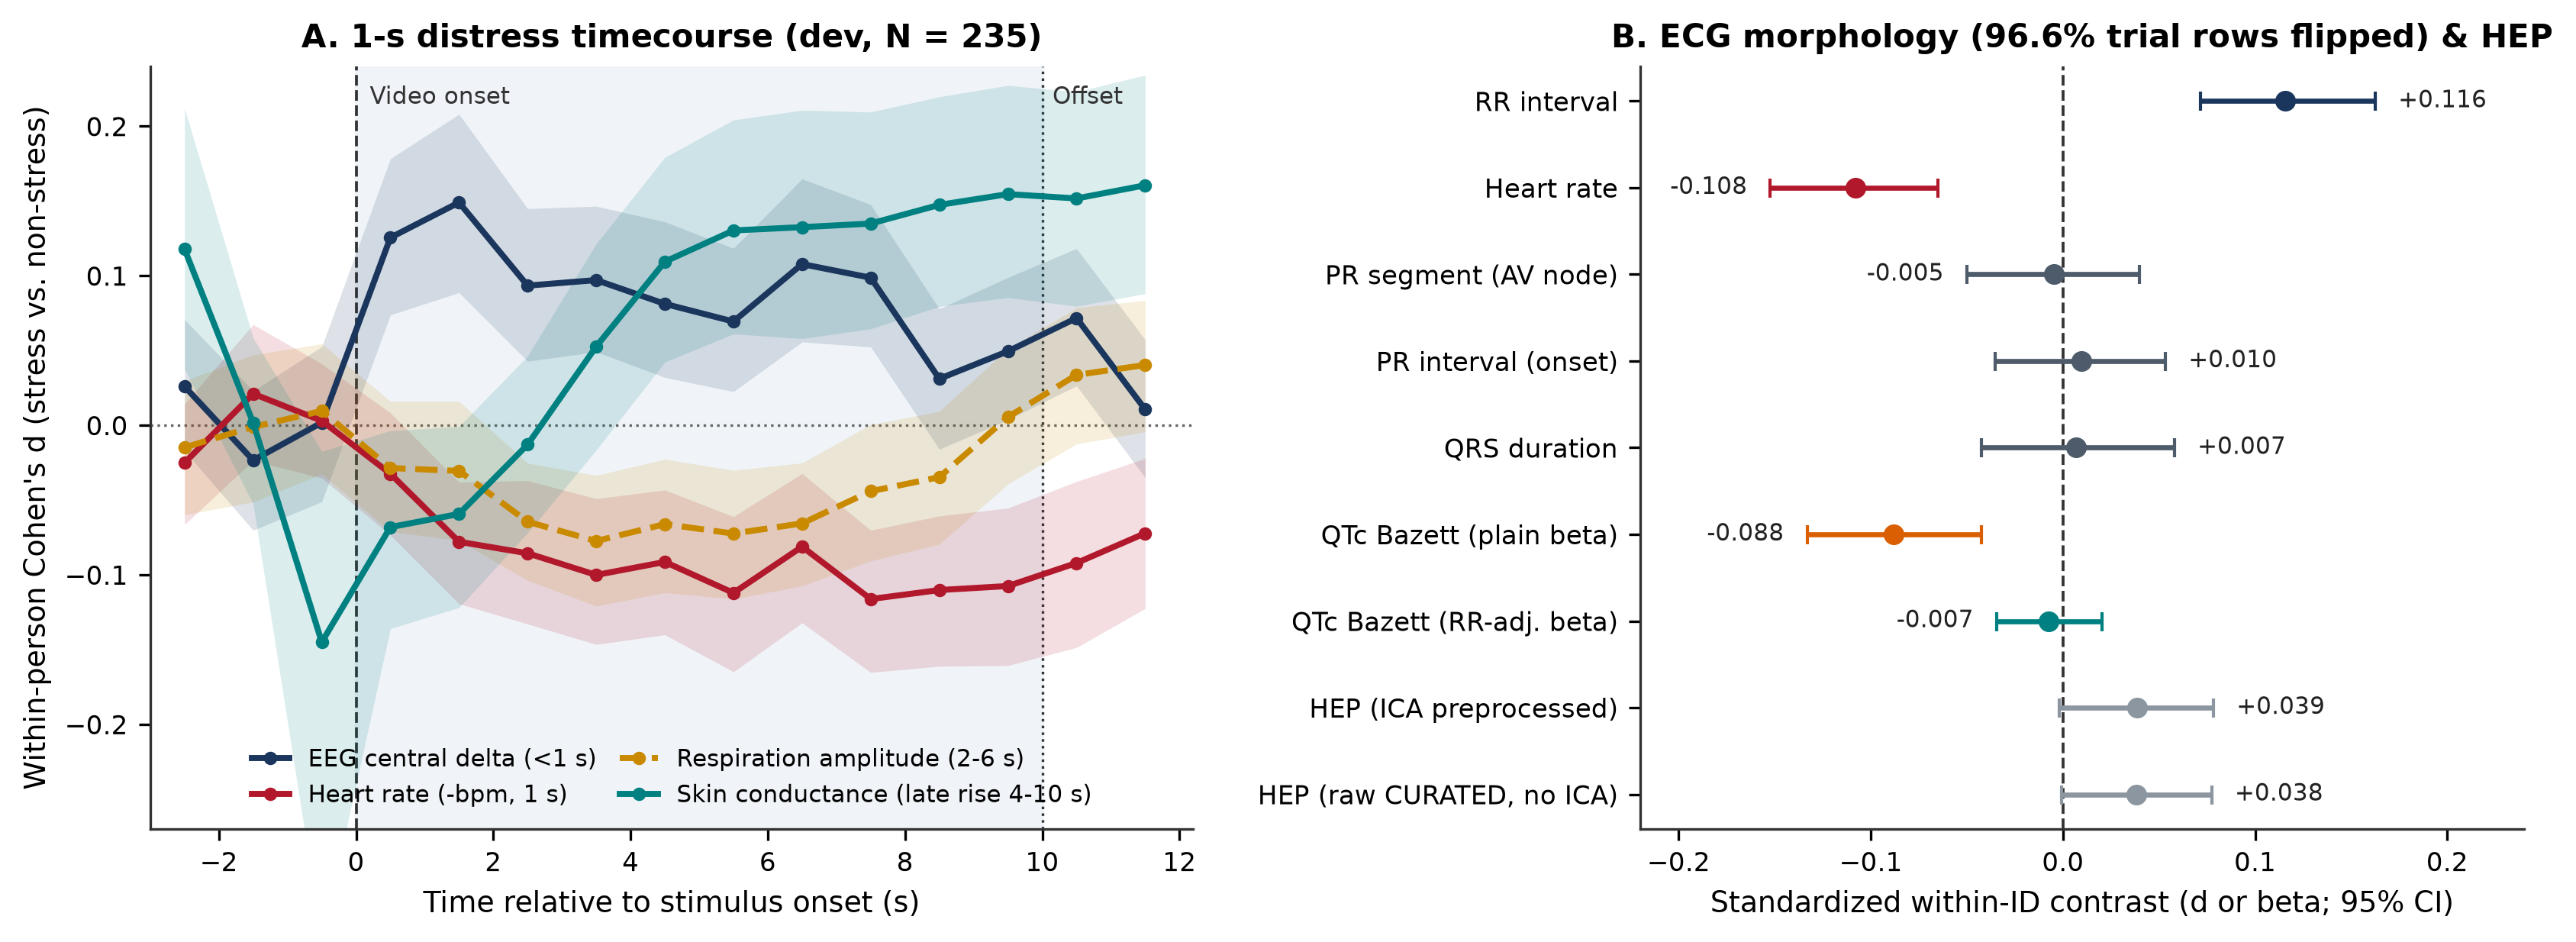
\includegraphics[width=0.89\textwidth]{figures/fig1_physiology_cascade.png}
\caption{\textbf{Cascade multimodale du stress aigu et morphologie ECG battement par battement.} (A) Taille d'effet intra-sujet ($d$ de Cohen) par pas de 1\,s ($[-3, 12)\,\text{s}$, zone gris\'ee : clip) : EEG delta ($<1\,\text{s}$), fr\'equence cardiaque ($1\,\text{s}$), respiration ($2\text{--}6\,\text{s}$) et conductance cutan\'ee ($4\text{--}10\,\text{s}$). (B) Intervalles ECG apr\`es correction automatique de polarit\'e Lead~I (96{,}6\,\% invers\'es) et HEP brut contre ICA : RR s'allonge ($+0{,}116$), segment PR nul ($-0{,}005$), baisse QTc Bazett ($-0{,}088$) annul\'ee apr\`es contr\^ole de $\Delta\text{RR}$ ($-0{,}007$), HEP brut CURATED \'egal au HEP ICA (nuls).}
\label{fig:phys}
\end{figure*}

La d\'elin\'eation ECG (figure~\ref{fig:phys}B) pr\'ecise la r\'eponse cardiaque. Pendant le stress aigu, l'intervalle RR s'allonge de $+5{,}06\,\text{ms}$ ($d = +0{,}116$, IC 95\,\% $[+0{,}071, +0{,}163]$), alors que le segment PR ($d = -0{,}005$, $[-0{,}047, +0{,}036]$), l'intervalle PR ($+0{,}010$) et le QRS ($+0{,}007$) ne varient pas. Le QTc Bazett brut baisse ($d = -0{,}088$), mais contr\^oler $\Delta\text{RR}$ au sein du sujet annule l'effet ($d = -0{,}007$, $[-0{,}035, +0{,}020]$). Ce profil est compatible avec une d\'ec\'el\'eration cardiaque \`a m\'ediation vagale au n{\oe}ud sino-atrial \cite{somsen2002}, sans variation mesurable de conduction AV ni de repolarisation ventriculaire propre sur 10\,s. Le HEP \texttt{CURATED} brut ($d = +0{,}038$, $[-0{,}001, +0{,}077]$) co\"incide avec le HEP ICA ($d = +0{,}039$, $[-0{,}002, +0{,}078]$), sans indice d'un signal masqu\'e par l'ICA.

Maintenir la vid\'eo fixe tout en contr\^olant le d\'es\'equilibre de classe s\'epare orientation sensorielle automatique et \'evaluation subjective. Sur 48 clips polarisants r\'eunissant des spectateurs stress\'es et tr\`es calmes ($V \ge 6 \cap A \le 4$), l'AUC intra-clip passe de $0{,}525$ (tous non-stress) \`a $0{,}564$, et l'\'evaluation subjective appari\'ee d\'eplace la fr\'equence cardiaque de $-2{,}97\,\text{bpm}$ ($d = -0{,}41$). Les sujets restant calmes devant un clip aversif ne montrent aucun changement de FC ni d'EDA ($-0{,}49\,\text{bpm}$, $+0{,}014\,\mu\text{S}$) ; seule la baisse d'alpha occipital persiste automatiquement ($d = -0{,}33$ \`a $-0{,}41$), marquant l'engagement attentionnel et la vigilance face \`a la menace plut\^ot que le stress ressenti \cite{codispoti2023,stegmann2024}. \`A clip identique ($N = 209$), la comparaison peur contre d\'ego\^ut confirme l'h\'et\'erog\'en\'eit\'e des \'emotions n\'egatives sur 10\,s \cite{qin2023} : le d\'ego\^ut domine en delta pr\'ecoce ($d = -0{,}098$) et gamma frontal tardif ($-0{,}178$, prudence micro-EMG), tandis que la peur domine en baisse alpha tardive ($-0{,}137$), bradycardie tardive et hausse EDA tardive ($+0{,}193$ ; tardif moins pr\'ecoce $+0{,}303$). Le clustering non supervis\'e ne retrouve pas les \'etiquettes ($\text{ARI} < 0{,}009$).

\subsection{Audit des fuites et pr\'evision prospective cerveau-c{\oe}ur}
Notre audit r\'etrospectif a expos\'e deux fuites subtiles. Le centrage global par personne sur l'ensemble du jeu gonflait l'AUC logistique de $+0{,}0141$ ($0{,}5705$ contre $0{,}5564$ en Cold-Start). Par ailleurs, \'evaluer un encodeur \texttt{REVE} bidirectionnel sur 13\,s avec 77\,\% de th\`emes d\'ej\`a vus cr\'eait des gains inter-modaux illusoires ($+0{,}059$ FC, $+0{,}042$ EDA, $+0{,}069$ respiration).

\begin{table}[t]
\centering
\caption{Pr\'evision prospective par EEG pr\'ecoce ($[-3{,}2, 5{,}0)\,\text{s}$) de la physiologie future ($[5, 10)\,\text{s}$) en Cold-Start $3 \times 3$ ($N = 200\text{--}228$) et LOCO-CV (5 cohortes).}
\label{tab:forecast}
\scriptsize
\setlength{\tabcolsep}{2.8pt}
\begin{tabular}{@{}lcccc@{}}
\toprule
Cible / r\'egime & $M_0$ ($r$) & $\Delta r$ ($M_{2,\text{res}}$) & $\Delta r$ ($M_{2,\text{jnt}}$) & \% am\'el. \\
\midrule
Fr\'eq. card. $[5,10)\,\text{s}$ & 0{,}6849 & $+0{,}0089^*$ & $+0{,}0110^*$ & 71{,}4\,\% \\
FC (sensibilit\'e $5\times5$) & 0{,}6852 & $+0{,}0094^*$ & $+0{,}0120^*$ & 71{,}0\,\% \\
FC (GBDT non lin\'eaire) & 0{,}6908 & $+0{,}0063^*$ & n/a & 57{,}6\,\% \\
FC (LOCO 5/5 cohortes) & 0{,}6885 & $+0{,}0107^*$ & n/a & 68{,}8\,\% \\
Cond. cutan\'ee $[5,10)\,\text{s}$ & 0{,}8218 & $-0{,}0097$ & $-0{,}0296$ & 45{,}0\,\% \\
Respiration $[5,10)\,\text{s}$ & 0{,}6417 & $+0{,}0008$ & $+0{,}0010$ & 52{,}6\,\% \\
\bottomrule
\end{tabular}
\vspace{1pt}
\raggedright\scriptsize $^*$\,IC bootstrap 95\,\% excluant z\'ero et BH-FDR $q < 0{,}002$.
\end{table}

\begin{figure*}[t]
\centering
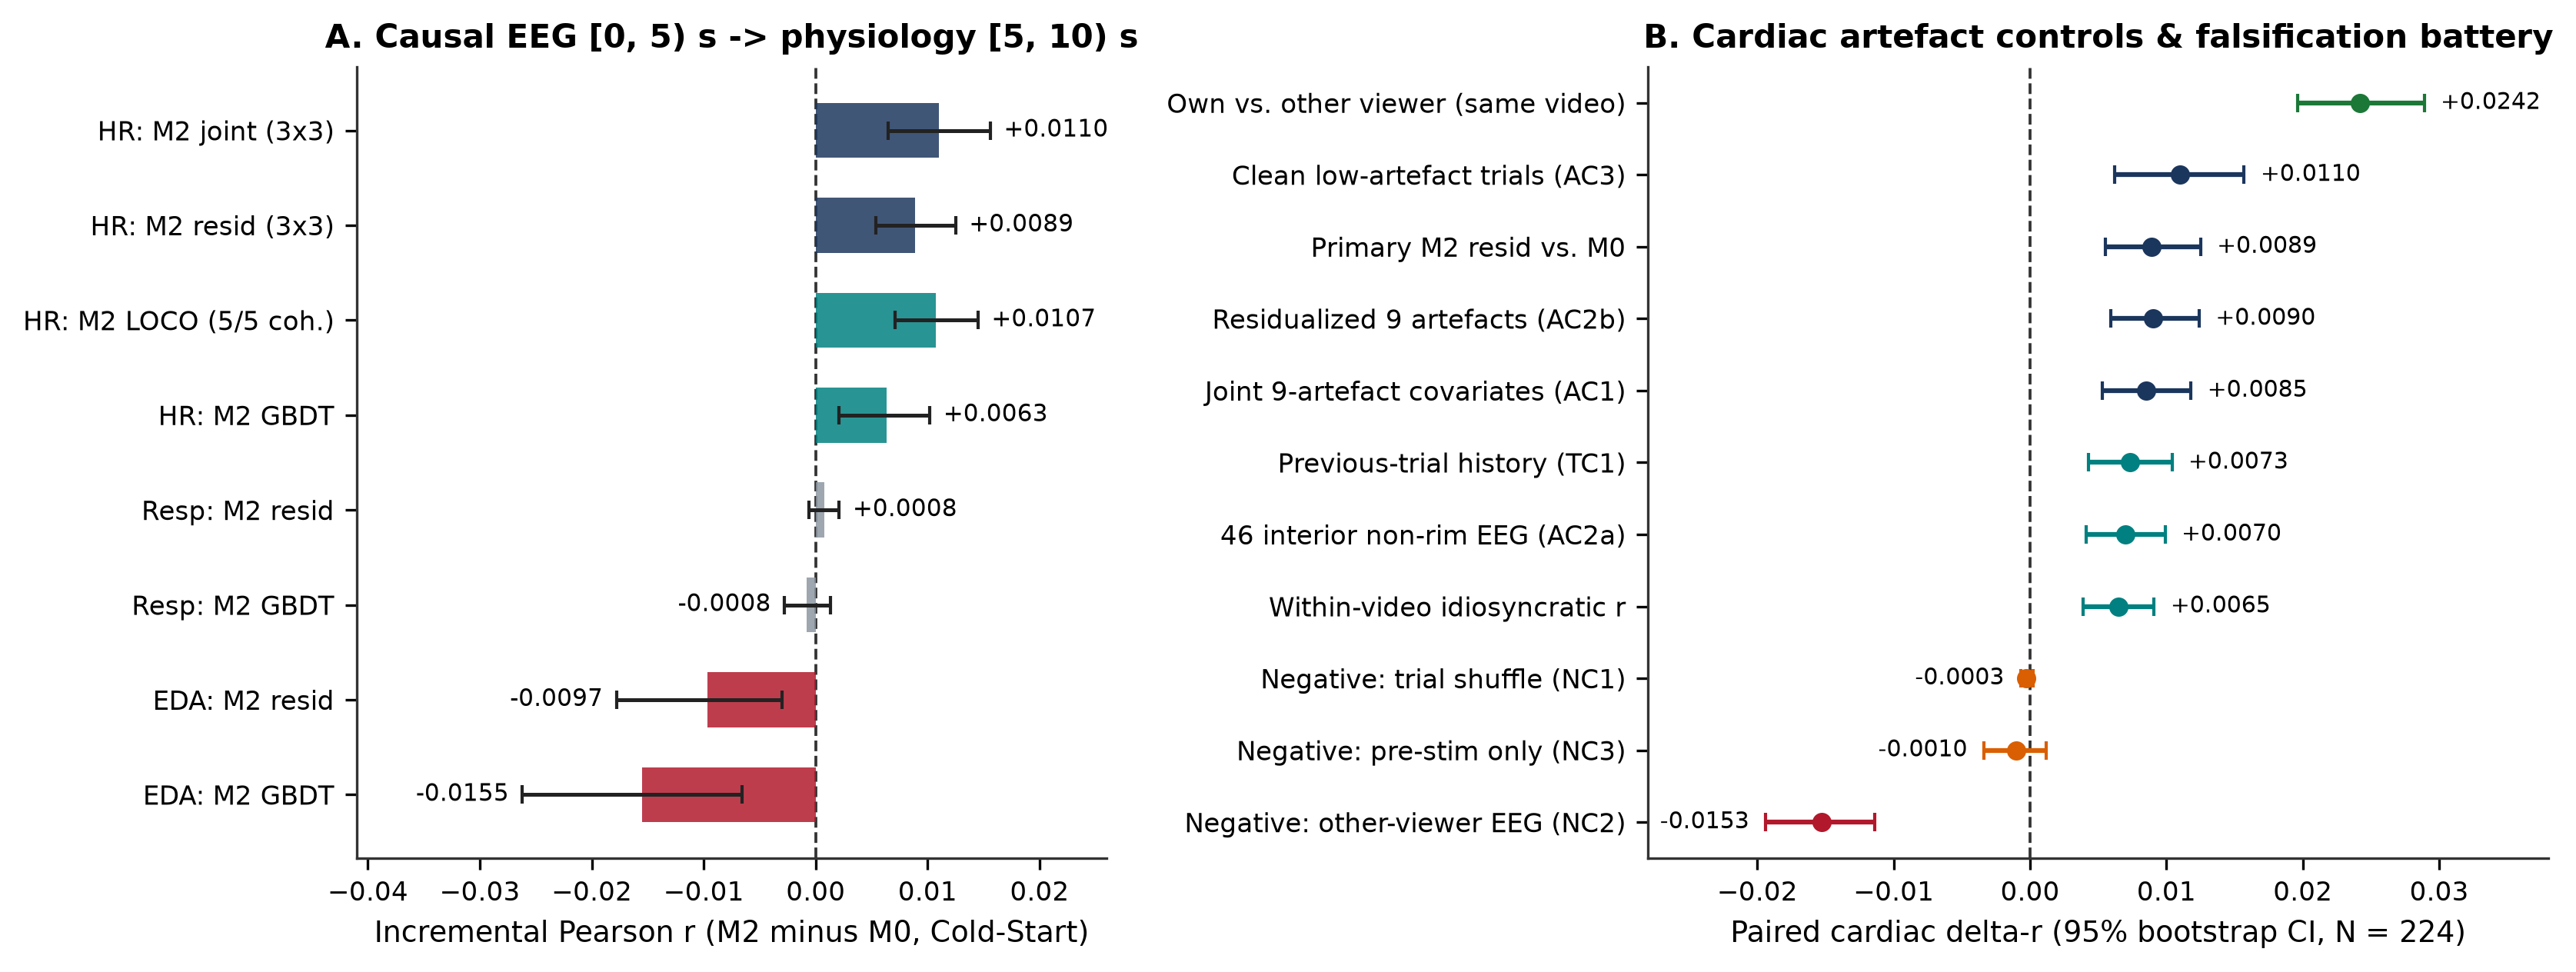
\includegraphics[width=0.89\textwidth]{figures/fig2_causal_brain_heart.png}
\caption{\textbf{Pr\'evision prospective EEG pr\'ecoce vers physiologie future (fronti\`ere $t = 5{,}000\,\text{s}$).} (A) Gain incr\'emental en corr\'elation de Pearson intra-sujet ($M_2 - M_0$, Cold-Start) par modalit\'e et en LOCO-CV sur 5 cohortes : gains cardiaques positifs en lin\'eaire, conjoint, GBDT et LOCO, aucun gain incr\'emental d\'etect\'e pour l'EDA ou la respiration. (B) Batterie de contr\^oles cardiaques ($N = 224$) : le gain persiste apr\`es 9 artefacts, 46 \'electrodes int\'erieures, essais propres, essai pr\'ec\'edent et test intra-vid\'eo, tombe \`a z\'ero sous permutation d'essais (NC1) et EEG pr\'e-stimulus (NC3), et favorise l'EEG propre face \`a un autre spectateur sur le m\^eme clip (NC2, $+0{,}0242$).}
\label{fig:causal}
\end{figure*}

Sous fronti\`ere temporelle \`a $t = 5{,}000\,\text{s}$, un gain pr\'edictif sp\'ecifique cerveau-c{\oe}ur persiste (tableau~\ref{tab:forecast}, figure~\ref{fig:causal}). L'EEG pr\'ecoce am\'eliore la pr\'evision cardiaque au-del\`a de $M_0$ ($r = 0{,}6849$) de $\Delta r = +0{,}0089$ ($[+0{,}0054, +0{,}0125]$, $M_{2,\text{res}}$) et $+0{,}0110$ ($[+0{,}0065, +0{,}0156]$, $M_{2,\text{jnt}}$, 71{,}4\,\% de sujets am\'elior\'es, $q < 10^{-6}$). Le gain demeure en $5 \times 5$ ($+0{,}0120$), en GBDT ($+0{,}0063$), sur l'incr\'ement pur $\Delta\text{FC}$ ($+0{,}0182$), avec garde de 2\,s ($+0{,}0089$) ou 5\,s ($+0{,}0038$), et se r\'eplique hors cohorte dans 5 cohortes HABS sur 5 en LOCO-CV ($+0{,}0107$, $[+0{,}0071, +0{,}0145]$, 68{,}8\,\% am\'elior\'es).

Tous les contr\^oles sont v\'erifi\'es (figure~\ref{fig:causal}B). Le gain cardiaque r\'esiste \`a l'ajout conjoint de neuf covariables EMG, EOG et mouvement ($+0{,}0085$), \`a leur r\'esidualisation ($+0{,}0090$), \`a la restriction aux 46 \'electrodes int\'erieures ($+0{,}0070$), aux essais propres ($+0{,}0110$) et \`a l'historique de l'essai pr\'ec\'edent ($+0{,}0073$). Les contr\^oles n\'egatifs s'annulent sous permutation intra-sujet (NC1 : $-0{,}0003$) et EEG pr\'e-stimulus seul (NC3 : $-0{,}0010$), et le m\'elange par blocs de 1\,s sur $[0, 5)\,\text{s}$ d\'egrade le signal (NC4 : $+0{,}0041$ r\'eel sur m\'elang\'e). Remplacer l'EEG d'un participant par celui d'un autre spectateur devant la m\^eme vid\'eo \'echoue (NC2 : $-0{,}0153$ ; propre moins autre $+0{,}0242$, 79\,\% am\'elior\'es), et la corr\'elation idiosyncratique intra-vid\'eo progresse de $+0{,}0065$. En revanche, aucun gain incr\'emental n'est d\'etect\'e pour l'EDA future ($-0{,}0097$, GBDT $-0{,}0155$) ni la respiration ($+0{,}0008$, GBDT $-0{,}0008$).

\subsection{Mod\`eles, g\'en\'eralisation, d\'erive et personnalisation}
Sur le protocole Cold-Start dev $3 \times 3$ audit\'e (tableau~\ref{tab:bench}), un mod\`ele Ridge 4 phases sans GPU atteint une AUC de $0{,}5709$ ($[0{,}5565, 0{,}5849]$). Il \'egale \texttt{EEGNet} supervis\'e ($0{,}5722$) et d\'epasse les cinq mod\`eles de fondation EEG pr\'e-entra\^in\'es (\texttt{S-JEPA} $0{,}526$, \texttt{LaBraM} $0{,}549$, \texttt{CBraMod} $0{,}556$, \texttt{REVE-base} $0{,}557\text{--}0{,}561$, \texttt{EEGPT} $0{,}560$), un \texttt{PhysioJEPA} multimodal entra\^in\'e sur HABS ($0{,}557$), le fine-tuning LoRA de \texttt{REVE} ($0{,}550$, $-0{,}0069$ face \`a la t\^ete gel\'ee pour $21{,}7\times$ le co\^ut GPU) et l'empilement OOF imbriqu\'e ($-0{,}0084$). La perte de classement intra-sujet s'av\`ere d\'eterminante pour les r\'eseaux ($+0{,}0406$ face \`a l'entropie crois\'ee seule), et le retrait bay\'esien empirique r\'eduit la variance identitaire dans \texttt{REVE} de 51\,\% \`a 37\,\% (s\'eparant trait stable et \'etat \cite{saviola2020}) tout en am\'eliorant la calibration (Brier $0{,}2479$).

\begin{table}[t]
\centering
\caption{Comparaison des mod\`eles et ablation capteurs en Cold-Start $3 \times 3$ audit\'e (dev, $N = 208$ sujets \'eligibles).}
\label{tab:bench}
\scriptsize
\setlength{\tabcolsep}{1.8pt}
\begin{tabular}{@{}lcc@{}}
\toprule
Mod\`ele ou sous-ensemble de capteurs & AUC & IC 95\,\% \\
\midrule
Ridge 4 phases (Tous, 0 GPU) & \textbf{0{,}5709} & $[0{,}5565, 0{,}5849]$ \\
\texttt{EEGNet} (supervis\'e, 3 graines) & 0{,}5722 & $[0{,}5553, 0{,}5902]$ \\
\texttt{REVE-base} lin\'eaire gel\'e (EEG) & 0{,}5609 & $[0{,}5451, 0{,}5769]$ \\
\texttt{EEGPT} lin\'eaire gel\'e (EEG) & 0{,}5596 & $[0{,}5446, 0{,}5742]$ \\
\texttt{PhysioJEPA} affin\'e & 0{,}5570 & $[0{,}5445, 0{,}5706]$ \\
\texttt{REVE-base} LoRA (21{,}7$\times$ GPU) & 0{,}5495 & $[0{,}5336, 0{,}5653]$ \\
\midrule
R4 : Tous capteurs (Ridge 4 phases) & 0{,}5688 & $[0{,}5534, 0{,}5835]$ \\
R4 : sans ECG / sans Resp & 0{,}5688 / 0{,}5665 & $[0{,}552, 0{,}584]$ \\
R4 : sans EDA / sans EEG & 0{,}5511 / 0{,}5404 & $[0{,}526, 0{,}565]$ \\
R4 seul : EDA / EEG / Resp / ECG & \multicolumn{2}{c}{0{,}555 / 0{,}551 / 0{,}522 / 0{,}508} \\
\bottomrule
\end{tabular}
\end{table}

\begin{figure*}[t]
\centering
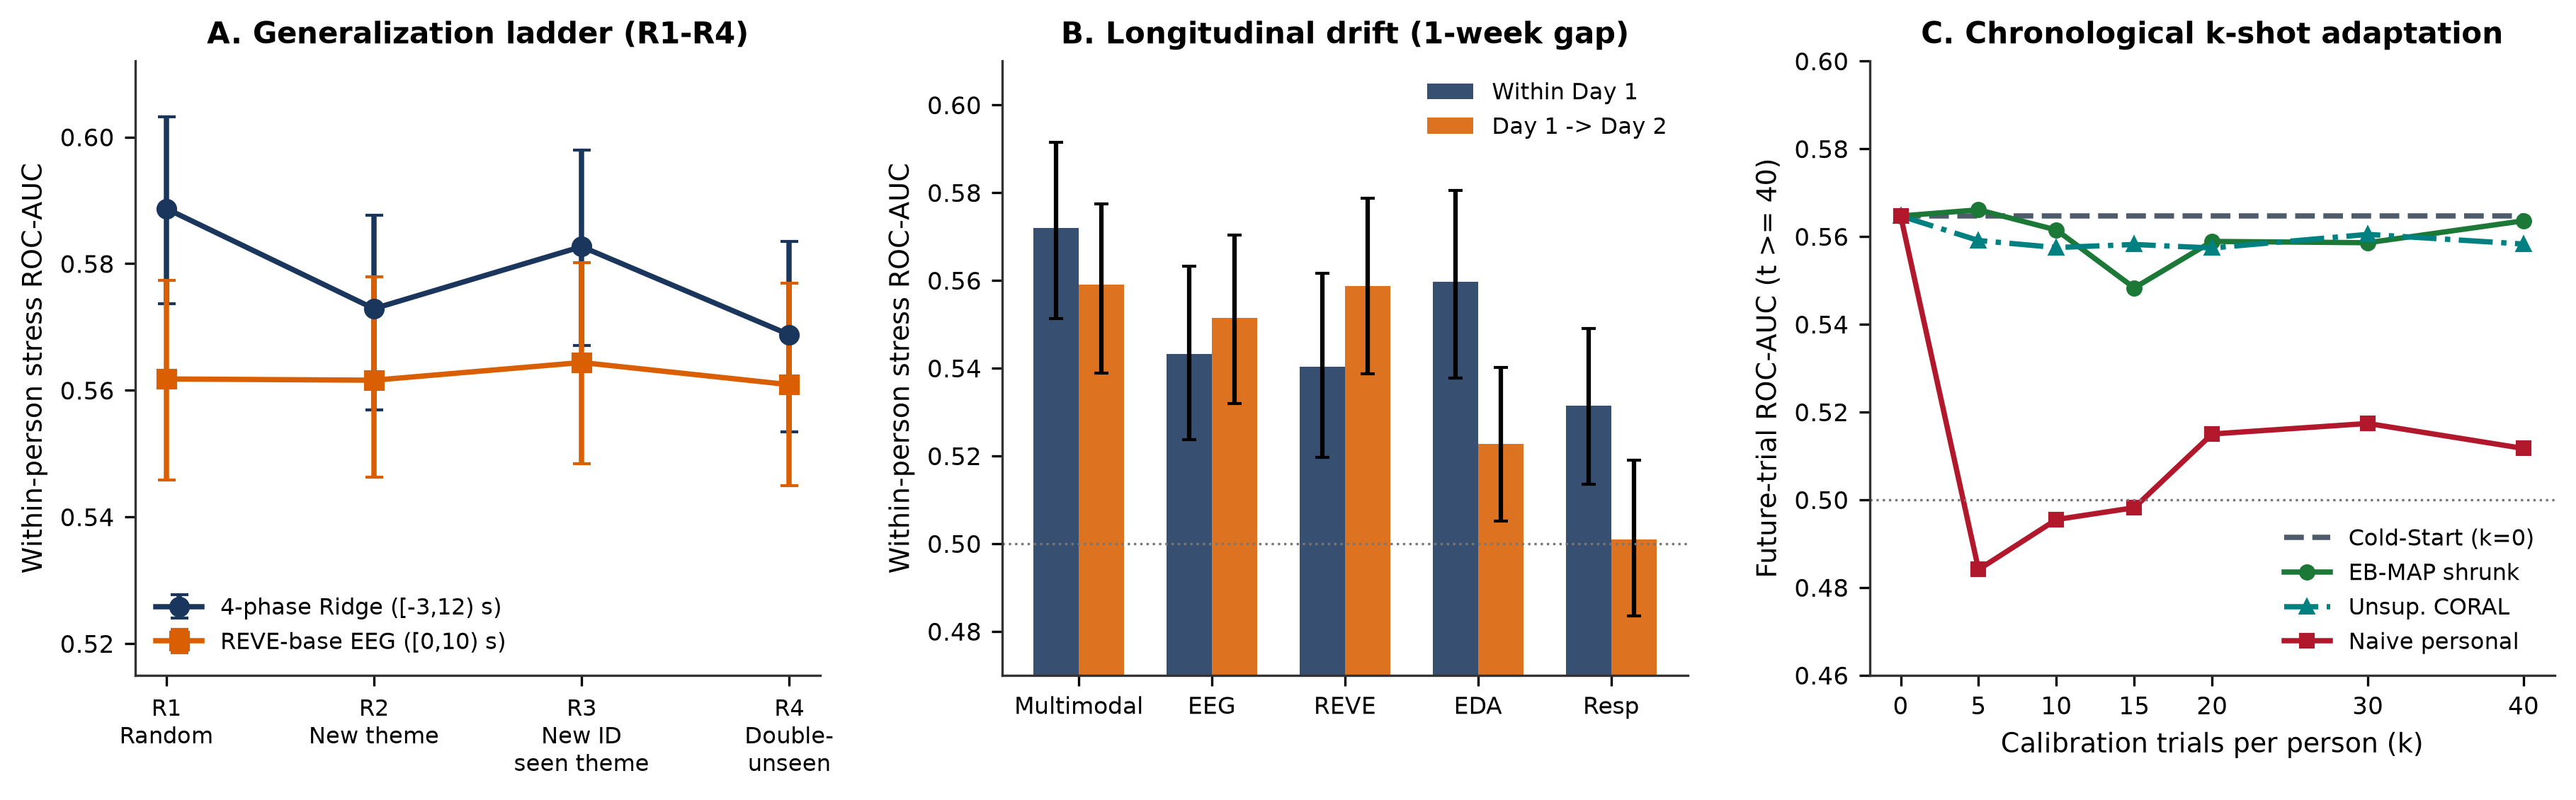
\includegraphics[width=0.91\textwidth]{figures/fig3_generalization_drift.png}
\caption{\textbf{\'Echelle de g\'en\'eralisation, d\'erive inter-jours et adaptation $k$-shot chronologique.} (A) L'AUC intra-sujet chute du split al\'eatoire (R1 : $0{,}5887$) au double non-vu Cold-Start (R4 : $0{,}5688$) ; 70\,\% de l'\'ecart viennent des th\`emes vus (R3$-$R4 $= +0{,}0139$). (B) \`A une semaine d'intervalle (Jour~1 $\to$ Jour~2, $N = 149$), l'EDA seule chute ($0{,}560 \to 0{,}523$, $-0{,}039$) et la respiration retombe au hasard ($0{,}501$), alors que l'EEG et le multimodal tiennent. (C) Personnalisation chronologique $k$-shot ($k = 0\text{--}40$) : le r\'eentra\^inement personnel na\"if s'effondre ($-0{,}081$ \`a $k = 5$), tandis que le retrait EB-MAP reste stable.}
\label{fig:gen}
\end{figure*}

La figure~\ref{fig:gen} d\'ecompose trois obstacles au d\'eploiement. Sur l'\'echelle de g\'en\'eralisation (figure~\ref{fig:gen}A), passer d'une CV al\'eatoire (R1 : $0{,}5887$) au double non-vu Cold-Start (R4 : $0{,}5688$) retire $0{,}0199$ d'AUC, prolongeant les observations LOSO contre al\'eatoire \cite{alshamrani2026} en montrant que 70\,\% proviennent des th\`emes vus (R3 LOSO th\`emes vus $= 0{,}5827$ ; R3$-$R4 $= +0{,}0139$). En score agr\'eg\'e hors \'evaluation intra-sujet, la r\'egression logistique sur \texttt{REVE} subit une inflation biom\'etrique suppl\'ementaire de $+0{,}0408$. En R4, l'ablation confirme que l'EEG ($-0{,}0284$) et l'EDA ($-0{,}0177$) forment les deux piliers compl\'ementaires, l'ECG seul restant pr\`es du hasard ($0{,}5075$).

Le transfert \`a une semaine (figure~\ref{fig:gen}B) expose une forte d\'erive p\'eriph\'erique \cite{sakimura2025}. L'EDA tonique est peu stable d'un jour \`a l'autre ($r = 0{,}420$), les SCR phasiques s'habituent en s\'eance ($d = -0{,}032$) alors que le RR vagal ne s'habitue pas ($+5{,}66\,\text{ms}$, en accord avec des cin\'etiques d'habituation distinctes \cite{chen2014}), et l'\texttt{EDA\_only} perd $-0{,}0392$ d'AUC du Jour~1 ($0{,}5597$) au Jour~2 ($0{,}5228$), tandis que la \texttt{Resp\_only} chute de $-0{,}0299$ au hasard ($0{,}5010$). L'EEG seul ($0{,}543 \to 0{,}552$) et le mod\`ele multimodal ($0{,}572 \to 0{,}559$) se maintiennent.

La calibration chronologique $k$-shot ($k = 0\text{--}40$, \'evalu\'ee strictement sur les essais $t \ge 40$ ; figure~\ref{fig:gen}C) montre que le r\'eentra\^inement personnel na\"if s'effondre ($-0{,}0806$ d'AUC \`a $k = 5$, encore $-0{,}0531$ \`a $k = 40$, et $-0{,}040$ \`a $-0{,}069$ entre jours). CORAL non supervis\'e \cite{sun2016,mihirette2025} est neutre en LOCO-CV ($0{,}589 \to 0{,}588$) et l\'eg\`erement n\'egatif en calibration courte ($-0{,}0055$). Le retrait MAP bay\'esien empirique vers les poids de population \'elimine l'effondrement sur tout $k$ et \'egale le Cold-Start.

\begin{figure*}[t]
\centering
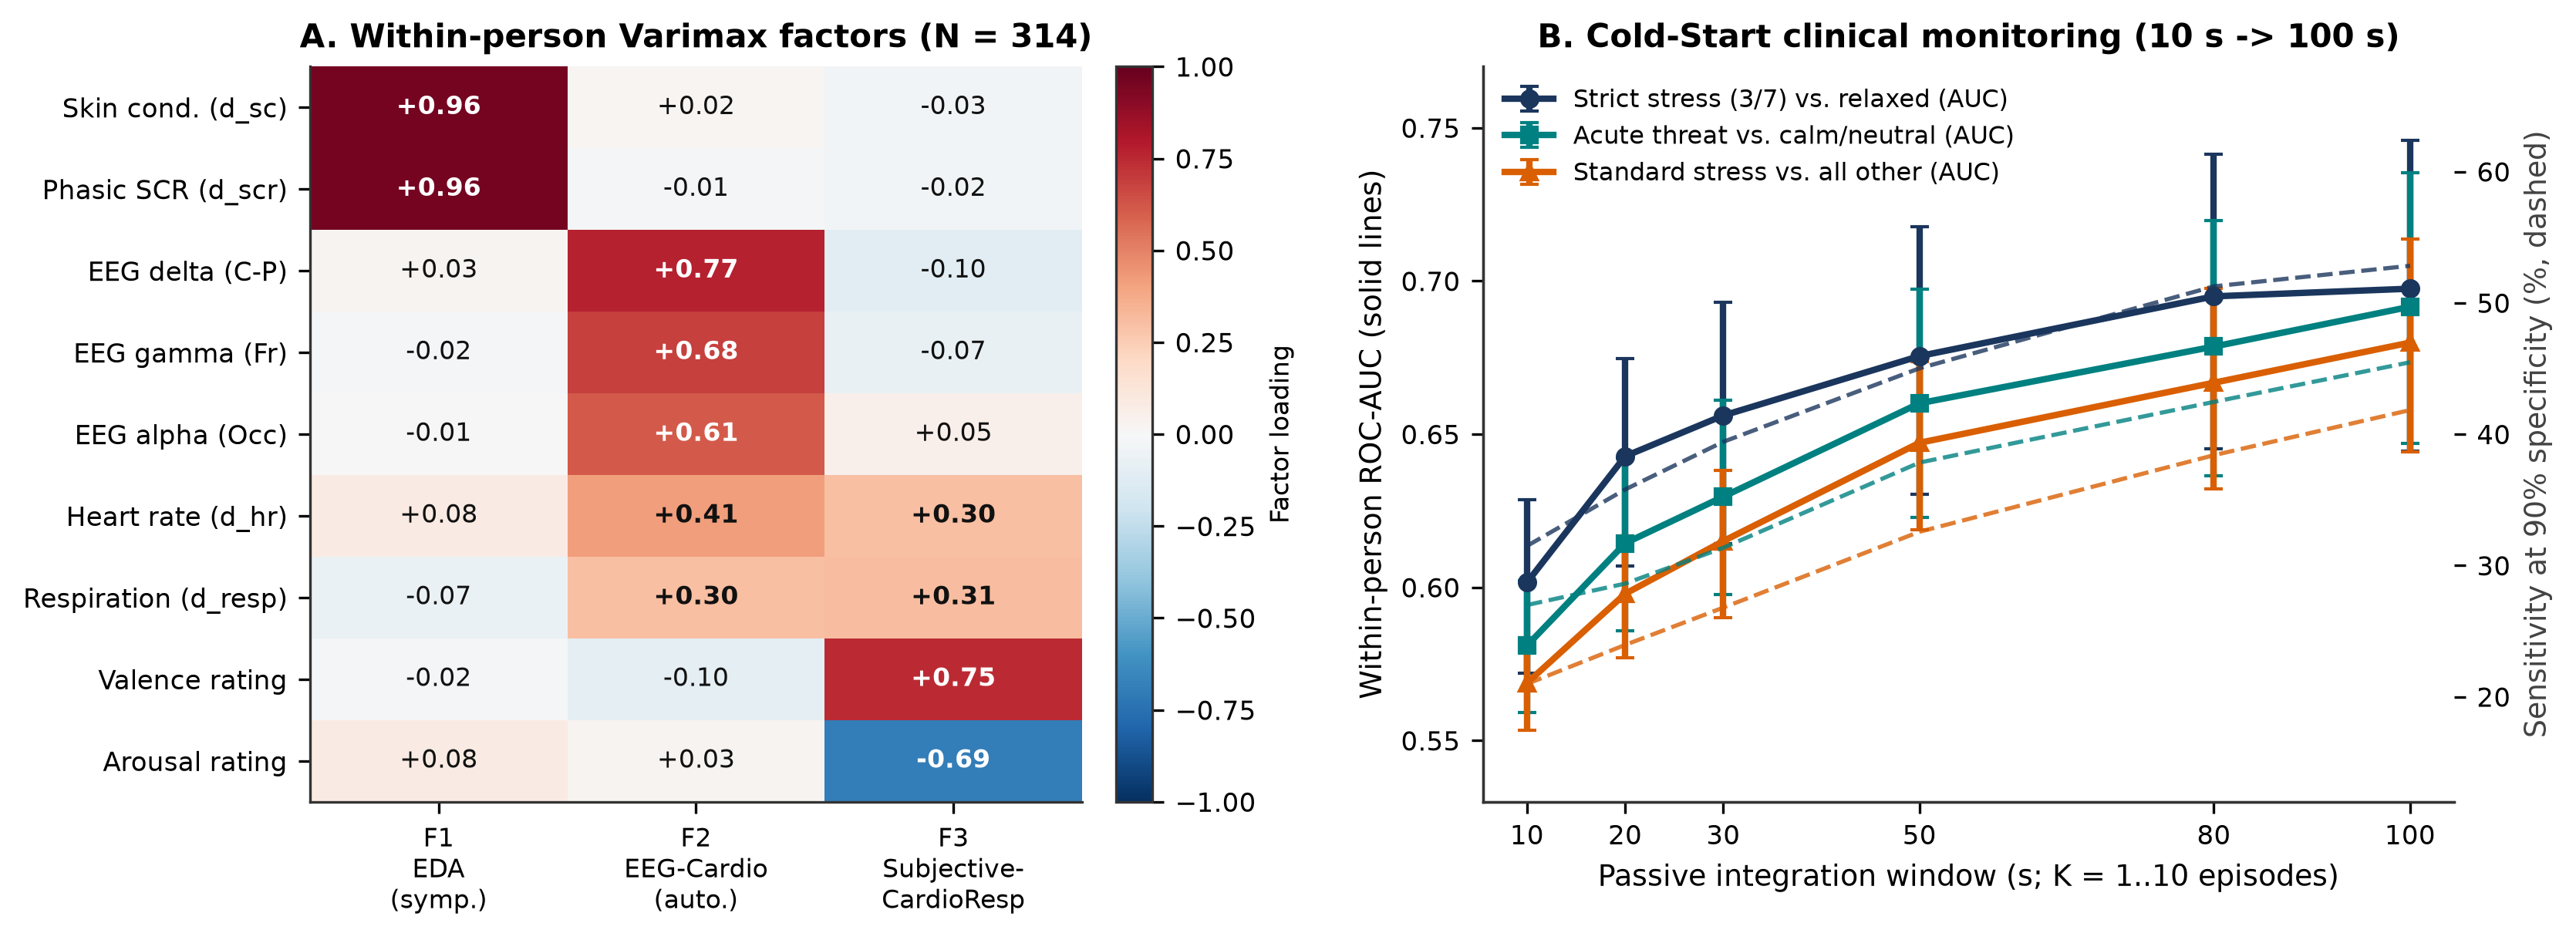
\includegraphics[width=0.89\textwidth]{figures/fig4_coherence_monitoring.png}
\caption{\textbf{Espace de divergence subjectif-autonome et courbes exp\'erimentales de suivi passif.} (A) Saturations Varimax \`a 3 facteurs intra-sujet sur 314 participants (16\,276 essais) s\'eparant EDA (F1), couplage automatique EEG-cardio-respiratoire (F2) et notes subjectives associ\'ees \`a FC/Resp (F3). (B) L'agr\'egation de scores Cold-Start R4 sur $K = 1\text{--}10$ clips discrets de m\^eme classe ($10\text{--}100\,\text{s}$ cumul\'ees) \'el\`eve l'AUC de $+0{,}10\text{--}0{,}11$ jusqu'\`a $0{,}680\text{--}0{,}698$ et double la sensibilit\'e \`a 90\,\% de sp\'ecificit\'e ($21\,\% \to 42\text{--}53\,\%$).}
\label{fig:mon}
\end{figure*}

\subsection{Divergence subjectif-autonome et suivi passif simul\'e}
L'analyse factorielle Varimax sur les 314 participants (16\,276 essais complets ; 53{,}3\,\% de variance expliqu\'ee ; figure~\ref{fig:mon}A) \'etend l'espace de divergence subjectif-autonome \cite{cuve2023} en trois axes orthogonaux : \textbf{F1 EDA sympathique} ($\Delta\text{SC}$ $+0{,}96$, $\Delta\text{SCR}$ $+0{,}96$), \textbf{F2 Cortico-cardio-respiratoire} (EEG $\delta$ $+0{,}77$, $\gamma$ $+0{,}68$, $\alpha$ $+0{,}61$, FC $+0{,}41$, Resp $+0{,}30$, avec saturations des notes $|<0{,}10|$) et \textbf{F3 Subjectif-cardio-respiratoire} (Valence $+0{,}75$, Activation $-0{,}69$, FC $+0{,}30$, Resp $+0{,}31$). La coh\'erence composite subjectif-physiologie ($\rho$ m\'edian $= +0{,}111$) est positive chez 79{,}0\,\% des sujets et nulle ou n\'egative ($\rho \le 0$) chez 21{,}0\,\%, et augmente lors des essais de forte intensit\'e ($+0{,}101$, r\'epliquant \cite{brown2019}). Aucune association statistiquement significative n'est observ\'ee entre le gain prospectif cerveau-c{\oe}ur ($M_2 - M_0$) et la coh\'erence subjective ($\rho = +0{,}091$, $p = 0{,}18$).

La figure~\ref{fig:mon}B montre l'effet de l'agr\'egation multi-\'episodes sur la d\'etection passive Cold-Start. Sur un clip isol\'e de 10\,s ($K = 1$), l'AUC vaut $0{,}569$ (standard), $0{,}581$ (menace aigu\"e contre calme/neutre) et $0{,}602$ (strict $3/7$ contre d\'etendu), pour une sensibilit\'e \`a 90\,\% de sp\'ecificit\'e de $21\text{--}32\,\%$. Moyenner $K = 10$ clips discrets de m\^eme classe ($100\,\text{s}$ cumul\'ees, bootstrap avec remise) \'el\`eve l'AUC de $+0{,}10\text{--}0{,}11$ \`a $0{,}680$ ($[0{,}644, 0{,}714]$), $0{,}692$ ($[0{,}647, 0{,}735]$) et $0{,}698$ ($[0{,}644, 0{,}746]$), portant la sensibilit\'e \`a 90\,\% de sp\'ecificit\'e \`a $41{,}8\,\%$, $45{,}5\,\%$ et $52{,}8\,\%$ ($59{,}2\,\%$ \`a 80\,\% de sp\'ecificit\'e). Les blocs disjoints sans remise confirment la progression lorsque les effectifs le permettent : \`a $K = 5$ ($50\,\text{s}$ cumul\'ees), l'AUC disjointe atteint $0{,}634$ ($N = 148$, standard) et $0{,}696$ ($N = 86$, menace aigu\"e) ; pour strict $3/7$ contre d\'etendu, elle atteint $0{,}658$ \`a $K = 3$ ($N = 88$) avant de se r\'etr\'ecir \`a $K = 5$ ($0{,}604$, $[0{,}513, 0{,}690]$, $N = 49$).

\section{Discussion}
\subsection{Port\'ee des r\'esultats}
\textbf{Neurophysiologie.} Sur des \'episodes aversifs de 10\,s, la r\'eactivit\'e cardiaque suit un profil compatible avec une d\'ec\'el\'eration vagale sans raccourcissement mesurable du segment PR ni variation du QT ind\'ependante de RR, et l'EEG pr\'ecoce porte une information pr\'edictive propre \`a chaque sujet sur la fr\'equence cardiaque future dans les cinq cohortes et apr\`es neuf contr\^oles d'artefacts. Aucun b\'en\'efice pr\'edictif incr\'emental n'a \'et\'e d\'etect\'e pour l'EDA ou la respiration, et les HEP bruts comme ICA ne montrent pas de modulation li\'ee au stress.

\textbf{M\'ethodologie Neuro-AI.} Les scores \'elev\'es rapport\'es sur de petits jeux affectifs masquent souvent des fuites par th\`emes vus, un contexte temporel bidirectionnel ou un centrage transductif. Une fois ces raccourcis \'elimin\'es, une r\'egression Ridge 4 phases interpr\'etable \'egale ou d\'epasse cinq mod\`eles de fondation EEG et un \texttt{PhysioJEPA} multimodal \`a co\^ut GPU nul. Les prochains travaux sur biosignaux devraient privil\'egier les pertes de classement intra-sujet et le retrait bay\'esien empirique plut\^ot que des mod\`eles plus lourds ou un r\'eentra\^inement personnel na\"if.

\textbf{Vers un suivi passif.} Les alertes isol\'ees sur 10\,s en z\'ero-shot sont trop bruit\'ees pour un usage au lit du patient. L'agr\'egation passive sur plusieurs \'episodes approche toutefois une AUC de $0{,}70$ et double la sensibilit\'e \`a haute sp\'ecificit\'e sans \'etiquettes de calibration. Associer EEG et EDA reste d\'ecisif : l'EDA renforce la d\'etection en s\'eance, tandis que l'EEG prot\`ege le syst\`eme contre la d\'erive et l'habituation \`a une semaine.

\subsection{Limites et p\'erim\`etre d'interpr\'etation}
Cinq limites encadrent ces conclusions. Premi\`erement, des adultes sains face \`a des vid\'eos de 10\,s forment un mod\`ele exp\'erimental et non une cohorte clinique ; le transfert \`a la douleur p\'ediatrique ou \`a la s\'edation en r\'eanimation exige une validation clinique directe sans pr\'esumer le m\^eme signe autonome, la douleur clinique induisant souvent une tachycardie sympathique plut\^ot qu'une bradycardie d'orientation \cite{danel2025,roue2025}. Deuxi\`emement, agr\'eger $K = 10$ clips discrets et non contigus de 10\,s simule une r\'eduction de bruit stationnaire sur 100 secondes cumul\'ees et n'\'equivaut pas \`a 100 secondes continues de suivi clinique, o\`u autocorr\'elation et d\'erive lente diff\`erent. Troisi\`emement, bien que tout le traitement post-release applique la s\'eparation personne par th\`eme, la normalisation par pli et le filtrage direct \`a $t = 5{,}000\,\text{s}$, l'EEG \texttt{PREPROCESSED} fourni par la release a subi une ICA et un filtrage amont sur l'enregistrement complet ; auditer un pr\'etraitement causal de bout en bout sur EEG brut reste une suite n\'ecessaire (partiellement \'eclair\'ee ici par le contr\^ole HEP sur \texttt{CURATED} brut et les 46 voies int\'erieures). Quatri\`emement, oculom\'etrie et pupillom\'etrie ont \'et\'e exclues pour d\'esalignement document\'e. Cinqui\`emement, nos r\'esultats n\'egatifs (HEP nul, gain EEG vers EDA/Resp non d\'etect\'e, CORAL neutre, effondrement $k$-shot na\"if et 21\,\% de discordance subjectif-autonome) fixent des limites r\'ealistes : les moniteurs physiologiques doivent compl\'eter, jamais remplacer, l'\'evaluation clinique et comportementale \cite{danel2025}.

\scriptsize
\shorthandoff{:}
\begin{thebibliography}{20}
\setlength{\itemsep}{0.5pt}
\bibitem{danel2025} A. Danel et al. Objective monitoring of acute pain and nociception in anaesthesia and intensive care. \emph{Anaesthesiol. Intensive Ther.} 57:213842, 2025.
\bibitem{roue2025} J.-M. Rou\'e et al. Objective detection of newborn infant acute procedural pain using EEG and machine learning algorithms. \emph{Paediatr. Neonatal Pain}, doi:10.1002/pne2.70001, 2025.
\bibitem{adama2025} V. S. Adama, M. Bogdan. Assessing consciousness in patients with locked-in syndrome using their EEG. \emph{Front. Neurosci.} 19:1604173, 2025.
\bibitem{somsen2002} R. J. M. Somsen, J. R. Jennings, M. W. van der Molen. Human vagal heart rate responses in warned reaction time tasks. \emph{J. Electrocardiol.} 35:131--138, 2002.
\bibitem{chen2014} K. H. Chen et al. Habituation of parasympathetic-mediated heart rate responses to recurring acoustic startle. \emph{Front. Psychol.} 5:1288, 2014.
\bibitem{munoz2015} M. L. Munoz et al. Validity of (ultra-)short recordings for heart rate variability measurements. \emph{PLOS ONE} 10:e0138921, 2015.
\bibitem{schippers2018} A. Schippers et al. Ultra-short term heart rate variability as a tool to assess changes in valence. \emph{Psychiatry Res.} 270:517--522, 2018.
\bibitem{parkblanke2019} H.-D. Park, O. Blanke. Heartbeat-evoked cortical responses: mechanisms, roles, and methodology. \emph{NeuroImage} 197:502--511, 2019.
\bibitem{engemann2018} D. A. Engemann et al. Robust EEG-based cross-site and cross-protocol classification of states of consciousness. \emph{Brain} 141:3179--3192, 2018.
\bibitem{alshamrani2026} M. Alshamrani. Cross-subject generalization in wearable physiological monitoring: four-class state classification. \emph{J. Eng. Res.}, S2307187726001586, 2026.
\bibitem{sakimura2025} M. Sakimura et al. Long-term variability in physiological-arousal relationships for robust emotion estimation. \emph{ACII}, arXiv:2508.18782, 2025.
\bibitem{mihirette2025} A. Mihirette et al. Cross-contextual stress prediction: comparing features and sample domain adaptation. \emph{Appl. Intell.} 55, doi:10.1007/s10489-025-06277-9, 2025.
\bibitem{brown2019} C. L. Brown et al. Coherence between subjective experience and physiology in emotion. \emph{Emotion} 20:818--829, 2020.
\bibitem{saviola2020} F. Saviola et al. Trait and state anxiety are mapped in the human brain. \emph{Sci. Rep.} 10:11112, 2020.
\bibitem{cuve2023} H. C. Cuve et al. Coherence and divergence in autonomic-subjective affective space. \emph{Psychophysiology} 61:e14461, 2024.
\bibitem{reve2025} J. O. El Ouahidi et al. REVE: A Foundation Model for EEG: Adapting to Any Setup with Large-Scale Pretraining. arXiv:2510.21585, 2025.
\bibitem{codispoti2023} M. Codispoti, A. De Cesarei, V. Ferrari. Alpha-band oscillations and emotion: a review of picture perception. \emph{Psychophysiology} 60:e14438, 2023.
\bibitem{stegmann2024} Y. Stegmann et al. Electrocortical responses in anticipation of avoidable and inevitable threats. \emph{J. Neurosci.} 44:PMC11484543, 2024.
\bibitem{qin2023} X. Qin et al. Different affective arousal and adaptation pattern between core and moral disgust. \emph{J. Psychol. Sci.} 46:320--328, 2023.
\bibitem{sun2016} B. Sun, J. Feng, K. Saenko. Return of frustratingly easy domain adaptation (CORAL). \emph{AAAI}, pp. 2058--2065, 2016.
\end{thebibliography}

\end{document}
